\documentclass{article}
\usepackage{graphicx} % 1. Load the graphicx package

\begin{document}

\section{My First Document with an Image}

Here is a picture of a cat, scaled to 50\% of its original size.

\begin{figure}[h!]
    \centering
    
\includegraphics[scale=0.5]{cat_picture2.png} % Change the filename here
    \caption{A cute cat}
    \label{fig:cat}
\end{figure}

The cat in Figure \ref{fig:cat} is very cute.

\section{My First Document with an Image}

Here is a picture of an interval chart, scaled to 50\% of its original size.

\begin{figure}[h!]
    \centering
    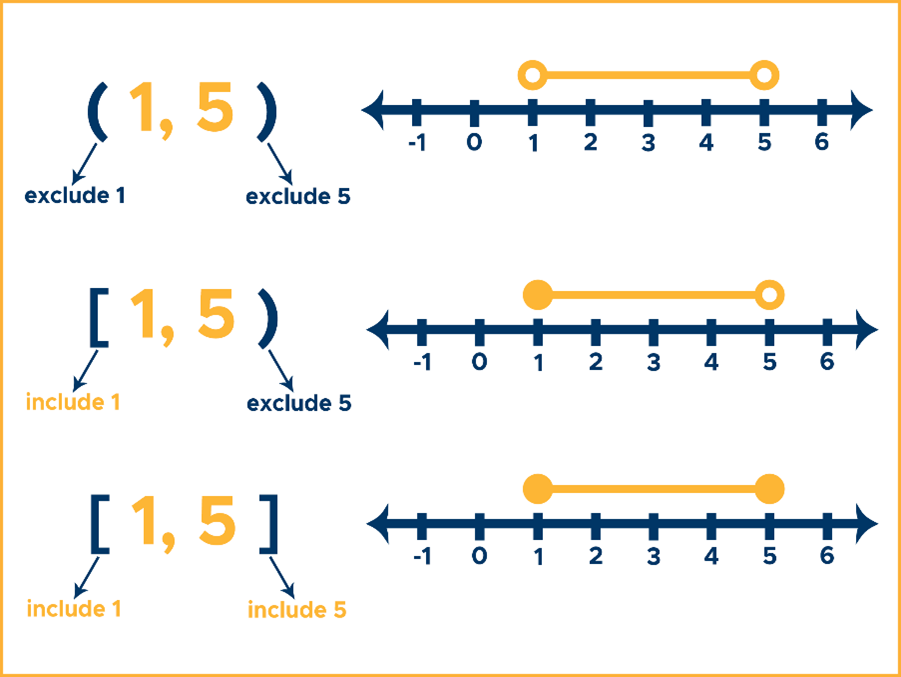
\includegraphics[scale=0.5]{Interval_chart.png} % Change the filename here
    \caption{An Interval Chart}
    \label{fig:cat}
\end{figure}

The cat in Figure \ref{fig:chart} is very cute.

\end{document}